\section{系统模型及理想成像仿真}
\subsection{成像系统模型和匹配滤波原理}
\begin{figure}[htb]
  \centering
  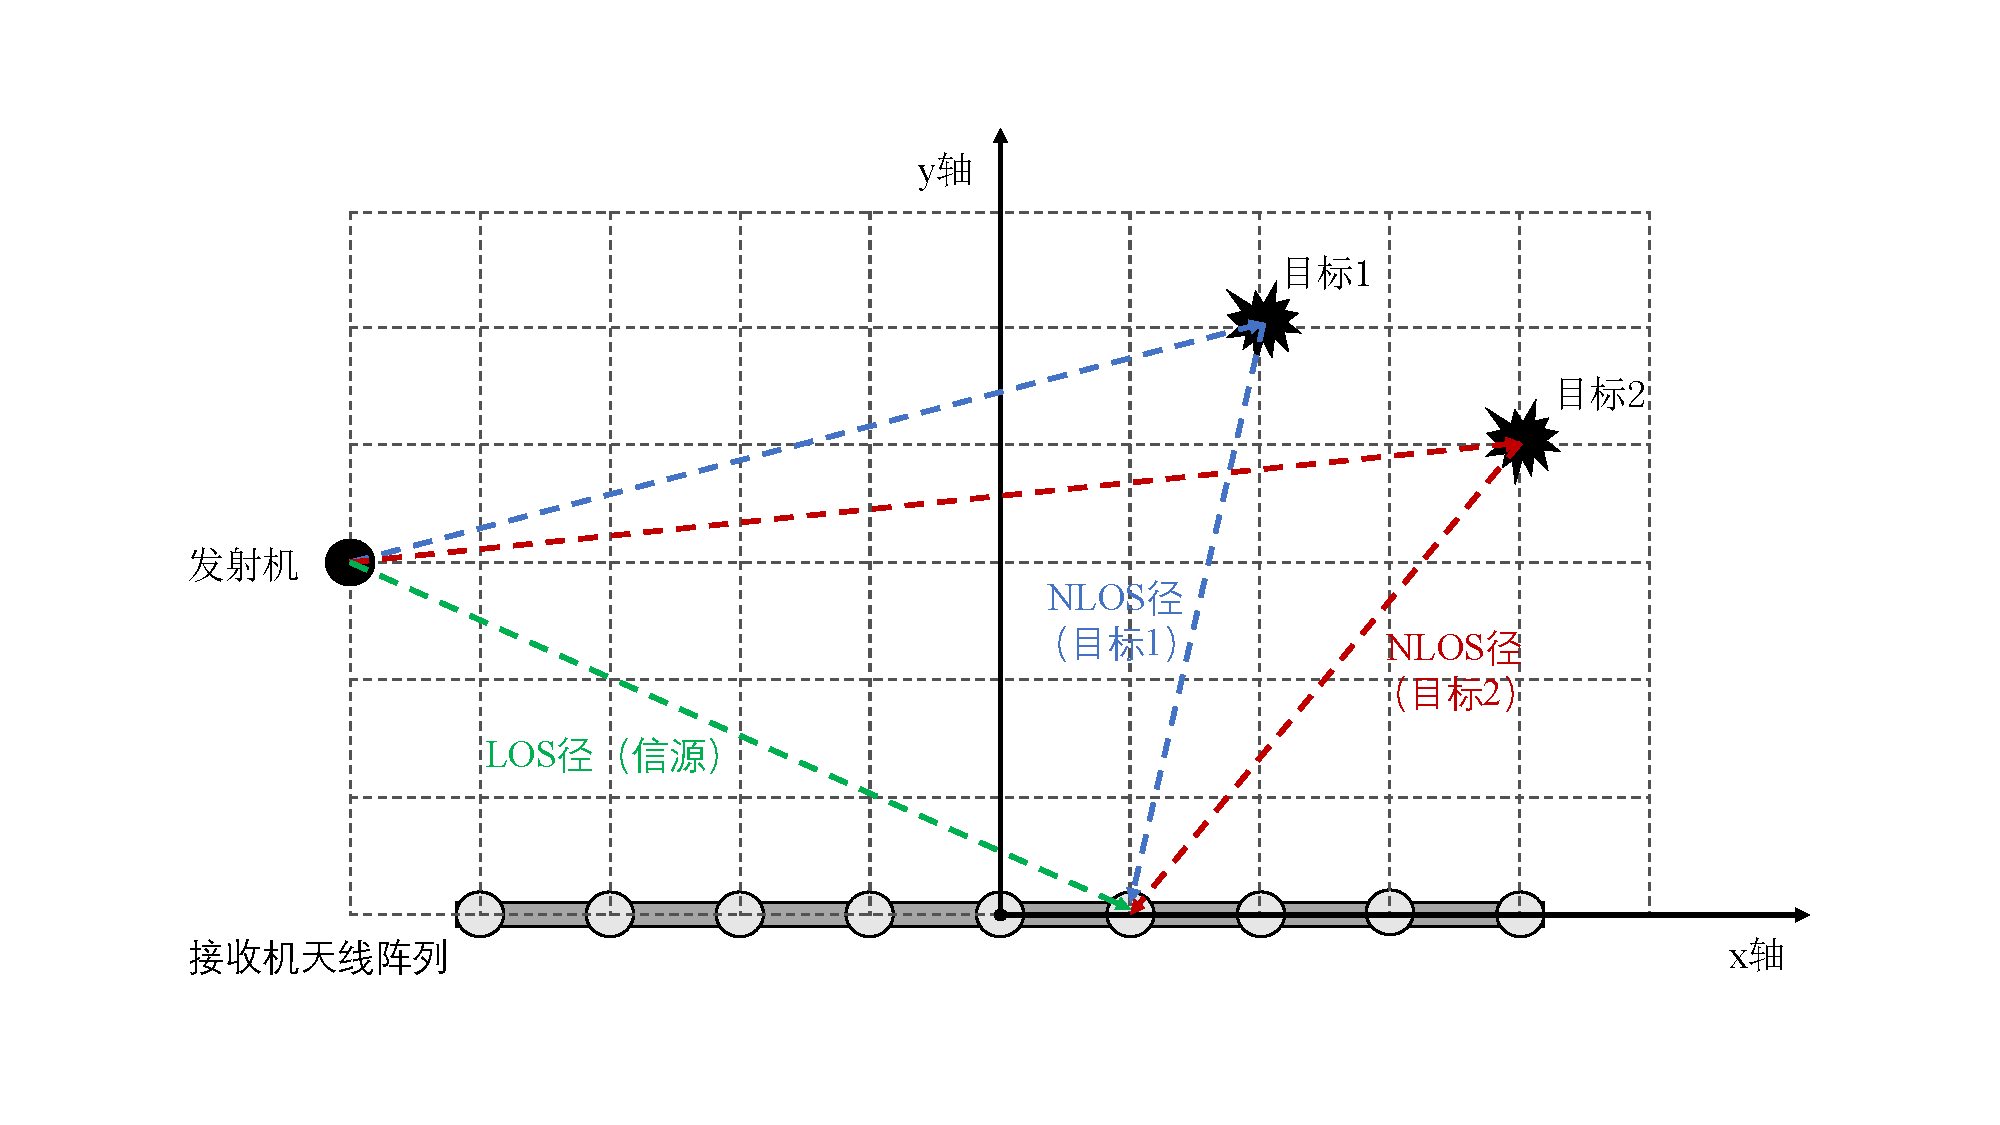
\includegraphics[width=\textwidth]{figures/system_model.pdf}
  \caption{系统模型}
  \label{系统模型}
\end{figure}
(\textbf{系统模型})图~\ref{系统模型}展示了本文所考虑的系统模型。为了方便叙述,这里先讨论的是单个发射机,单个接收机阵
列,两个目标的情形。我们将环境中的两个目标分别表示为:$\text{target}_1$ 和 $\text{target}_2$,设接收机阵列共有$N$个
阵元,并放置于如图的x轴之上。对于整个接收机天线阵列,对接收信号处理所得的CSI为$\boldsymbol{y}=[y_1,\cdots,y_n]^T$,其中第$n$个
阵元所接收的CSI可以表示为发射机对应的一条直射径(LOS: Line Of Sight)与目标对应的两条非直射径
(NLOS: Non Line Of Sight)的叠加\cite{ma2019wifi}:
\begin{align}
  y_n = \underbrace{\alpha_0(n)e^{-j2\pi\frac{d_0(n)}{\lambda}}}_{\text{LOS径}} + \underbrace{\alpha _1(n)e^{ - j2\pi \frac{D_1 + d_1(n)}{\lambda }} + \alpha _2(n)e^{ - j2\pi \frac{D_2 + d_2(n)}{\lambda }}}_{\text{NLOS 径}}\text{,}
\end{align}
其中,$\alpha_0$,$\alpha_1$与$\alpha_2$为幅度衰减因子。$D_1$和 $D_2$分别为发射机到$\text{target}_1$ 和 $\text{target}_2$的距离。$d_0(n)$,$d_1(n)$和$d_2(n)$分别为发射机,$\text{target}_1$和$\text{target}_2$到接收机第$n$个阵元的距离。$\lambda = c/f_c$为Wi-Fi信号的工作波长(在本文后续的仿真与实测中Wi-Fi信号的工作频率$f_c$取$4.2$GHz)。


(\textbf{匹配矩阵构造})将整个感知的平面网格化,针对每一个网格点,根据网格点$(x,y)$到第$n$个接收阵元的距离$(z_n,0)$
的距离$\hat{d}(n)=\sqrt{(x-z_n)^2+y^2}$,可得该网格点与第$n$个接收阵元的相位差为$2\pi\hat{d}(n)/\lambda$,将此设为
网格点$(x,y)$的相位纠正(需要注意的是,我们还可以根据信道衰落与距离的关系,做出相应的幅度补偿,为了便于分析,这里不再讨论)。因此,对于每一个网格点$(x,y)$,我们都有一个匹配向量:
\begin{align}
  \hat{\boldsymbol{y}}=[e^{j2\pi \hat{d}(1)/\lambda} ,\cdots,e^{j2\pi \hat{d}(N)/\lambda}]^T \text{,} \hat{d}(n)=\sqrt{(x-z_n)^2+y^2} \text{。}
  \label{matched array}
\end{align}


(\textbf{匹配滤波})对所有的网格点,将接收的阵列信号$\boldsymbol{y}$与其对应的$\hat{\boldsymbol{y}}$进行匹配,我们可以得到匹配结果:
\begin{align}
  & y_\text{match}  = \boldsymbol{y}^T\hat{\boldsymbol{y}} = \begin{bmatrix}
    \alpha_0(1)e^{-j2\pi\frac{d_0(1)}{\lambda}}+\alpha_1(1)e^{-j2\pi\frac{D_1+d_1(1)}{\lambda}}+\alpha_2(1)e^{-j2\pi\frac{D_2+d_2(1)}{\lambda}} \\
    \vdots \\
    \alpha_0(n)e^{-j2\pi\frac{d_0(n)}{\lambda}}+\alpha_1(n)e^{-j2\pi\frac{D_1+d_1(n)}{\lambda}}+\alpha_2(n)e^{-j2\pi\frac{D_2+d_2(n)}{\lambda}}
  \end{bmatrix}^T
  \begin{bmatrix}
    e^{j2\pi \hat{d}(1)/\lambda} \\
    \vdots \\
    e^{j2\pi \hat{d}(N)/\lambda}  
  \end{bmatrix} \nonumber \\
  & = \sum\limits_{n=1}^N \left(\alpha_0(n)e^{-j2\pi\frac{d_0(n)-\hat{d}(n)}{\lambda}}+\alpha_1(n)e^{-j2\pi\frac{D_1+d_1(n)-\hat{d}(n)}{\lambda}}+\alpha_2(n)e^{-j2\pi\frac{D_2+d_2(n)-\hat{d}(n)}{\lambda}}\right)\text{,}
\end{align}
为了便于分析,我们忽略幅度的影响(假设幅度补偿完美)。在此遍历过程中,有关系式:
\begin{align} 
  & |y_\text{match}| = \left|\sum\limits_{n=1}^N \left(e^{-j2\pi\frac{d_0(n)-\hat{d}(n)}{\lambda}}+e^{-j2\pi\frac{D_1+d_1(n)-\hat{d}(n)}{\lambda}}+e^{-j2\pi\frac{D_2+d_2(n)-\hat{d}(n)}{\lambda}}\right)\right| \nonumber
  \\ 
  & = \left| N + \sum\limits_{n=1}^N \left(e^{-j2\pi\frac{D_1+d_1(n)-\hat{d}(n)}{\lambda}}+e^{-j2\pi\frac{D_2+d_2(n)-\hat{d}(n)}{\lambda}}\right) \right| \text{ 如果}\hat{d}(n)=d_0(n)\text{,信源出现峰值} \nonumber \\
  & = \left| Ne^{-j2\pi\frac{D_1}{\lambda}} +  \sum\limits_{n=1}^N \left(e^{-j2\pi\frac{d_0(n)-\hat{d}(n)}{\lambda}}+e^{-j2\pi\frac{D_2+d_2(n)-\hat{d}(n)}{\lambda}}\right) \right| \text{ 如果}\hat{d}(n)=d_1(n)\text{,目标1出现峰值} \nonumber \\
  & = \left| Ne^{-j2\pi\frac{D_2}{\lambda}} +  \sum\limits_{n=1}^N \left(e^{-j2\pi\frac{d_0(n)-\hat{d}(n)}{\lambda}}+e^{-j2\pi\frac{D_1+d_1(n)-\hat{d}(n)}{\lambda}}\right) \right| \text{ 如果}\hat{d}(n)=d_2(n)\text{,目标2出现峰值} \nonumber \\
  & \approx N \text{,}
\end{align}
从上述公式可以看出,在网格点遍历的过程中,对应信源,目标的网格点会出现峰值,关于这一现象,我们会在小节2.3给出详细的仿真。
\subsection{理想仿真成像}
本小节,我们给出更加详细的理想仿真成像模型,将上一小节的情形扩展到了环境之中存在1个发射机和$L$个目标($\text{target}_1,\cdots,\text{target}_L$)的情况,我们有:
\begin{itemize}
  \item 天线信号的接收信号$\boldsymbol{y}=[y_1,\cdots,y_n]^T$可以表示为发射机对应的一条直射径和$L$条目标对应的非直射径的叠加:
  \begin{align}
    y_n &= \underbrace{\alpha_0(n)e^{-j2\pi\frac{d_0(n)}{\lambda}}}_{\text{LOS径}} + \underbrace{\alpha _1(n)e^{ - j2\pi \frac{D_1 + d_1(n)}{\lambda }} + \cdots + \alpha _L(n)e^{ - j2\pi \frac{D_L + d_L(n)}{\lambda }}}_{L\text{条NLOS 径}} \nonumber \\
    &= \sum_{l=0}^L \alpha_l e^{-j 2\pi \frac{D_l + d_l(n)}{\lambda}} \text{,}
  \end{align}
  这里$\{\alpha_l\}_{l\in \mathcal{L}}$,$\{D_l\}_{l\in \mathcal{L}}$,$\{d_l\}_{l \in \mathcal{L}}$分别指第$l$条多径的幅度衰减因子的集合,发射机到$\text{target}_l$的距离的集合($D_0 = 0$),$\text{target}_l$到接收机的距离的集合。$\mathcal{L}=\{0,1,\cdots,L\}$为多径的下标集合($l=0$指LOS径,对应信源)。
  \item 匹配矩阵$\hat{\boldsymbol{y}}$仍然保持公式~\eqref{matched array}的形式。
  \begin{itemize}
    \item 需要注意的是,这里的匹配矩阵只需要计算一次。
  \end{itemize}
  \item 同样忽略幅度影响,可得匹配的结果:
  \begin{align}
    &|y_{\text{match}}| = |\boldsymbol{y}^T\hat{\boldsymbol{y}}| = \left| \sum\limits_{n=1}^N \sum\limits_{l=0}^{L}e^{-j2\pi\frac{D_l+d_l(n)-\hat{d}(n)}{\lambda}} \right| \nonumber \\
    & = \left| N + \sum\limits_{n=1}^N\sum_{l \in \mathcal{L}/\{0\}}e^{-j2\pi\frac{D_l+d_l(n)-\hat{d}(n)}{\lambda}}  \right| \text{ 如果}\hat{d}(n)=d_0(n)\text{,信源出现峰值} \nonumber \\ 
    & = \cdots \nonumber \\
    & = \left| Ne^{-j2\pi D_i\lambda} + \sum\limits_{n=1}^N\sum_{l \in \mathcal{L}/\{i\}}e^{-j2\pi\frac{D_l+d_l(n)-\hat{d}(n)}{\lambda}}  \right| \text{ 如果}\hat{d}(n)=d_i(n)\text{,目标}i\text{出现峰值} \nonumber \\
    & = \cdots \nonumber \\
    & = \left| Ne^{-j2\pi D_L\lambda} + \sum\limits_{n=1}^N\sum_{l \in \mathcal{L}/\{L\}}e^{-j2\pi\frac{D_L+d_L(n)-\hat{d}(n)}{\lambda}}  \right| \text{ 如果}\hat{d}(n)=d_L(n)\text{,目标}L\text{出现峰值} \nonumber \\
    & \approx N \text{。}
  \end{align}
  \item 为了使成像峰值更加明显,我们后续还对成像结果进行了归一化以及加窗(汉明窗)处理。
\end{itemize}
\subsection{理想成像仿真结果}
本小节展示了理想状态下的成像仿真,仿真设置见表~\ref{理想成像仿真设置}:
\begin{table}[htb]
  % h-here,t-top,b-bottom,优先级依次下降
      \begin{center}
      % 居中
          \caption{理想成像仿真设置}\label{理想成像仿真设置}
          \begin{tabular}{lc} % 三线表不能有竖线,l-left,c-center,r-right
              \toprule
              %三线表-top 线
              参数 & 值 \\
              \midrule
              %三线表-middle 线
              是否考虑对信源(发射机)成像 & 否,仿真多径没有设置LOS径\\
              是否考虑CSI频偏的影响 & 否,该小节测试理想成像的结果\\
              成像目标数量    & 3\\
              成像目标的位置  & $(1\text{米},1\text{米})$,$(2\text{米},1.5\text{米})$,$(3\text{米},2\text{米})$ \\
              工作频点        & $4.2$GHz\\
              工作带宽      & 20MHz \\
              子载波数目      & 256\\
              发射机位置           & $(2\text{米},0\text{米})$\\
              接收机天线阵元数$N$      & $32$,$64$,$128$\\
              接收机天线阵元间隔    & 半波长(约$3.57$厘米)\\
              接收机位置           & 类似图~\ref{系统模型},阵列中心位于原点\\
              \bottomrule
              %三线表-底线
          \end{tabular}
      \end{center}
\end{table}

需要注意的是:
\begin{itemize}
  \item 仿真考虑类似图~\ref{系统模型}中的单接收机阵列对三个目标进行成像(最初没有考虑对信源成像,但其实信源的成像与目标的成像是等效的);
  \item 仿真其实只利用了一个子载波上的信号进行成像,如何利用多载波上的CSI联合成像以提升成像性能是一个可能的拓展方向。 
  \item 本小节的仿真并没有考虑CSI频偏的影响,旨在得到一个``完美的''理想成像结果,作为后续考虑频偏成像的上界作为对比。
\end{itemize}

理想成像仿真结果如图~\ref{理想成像仿真结果}所示:

\begin{figure}[htb]
  \centering
  \begin{subfigure}[t]{.45\linewidth}
      \centering
      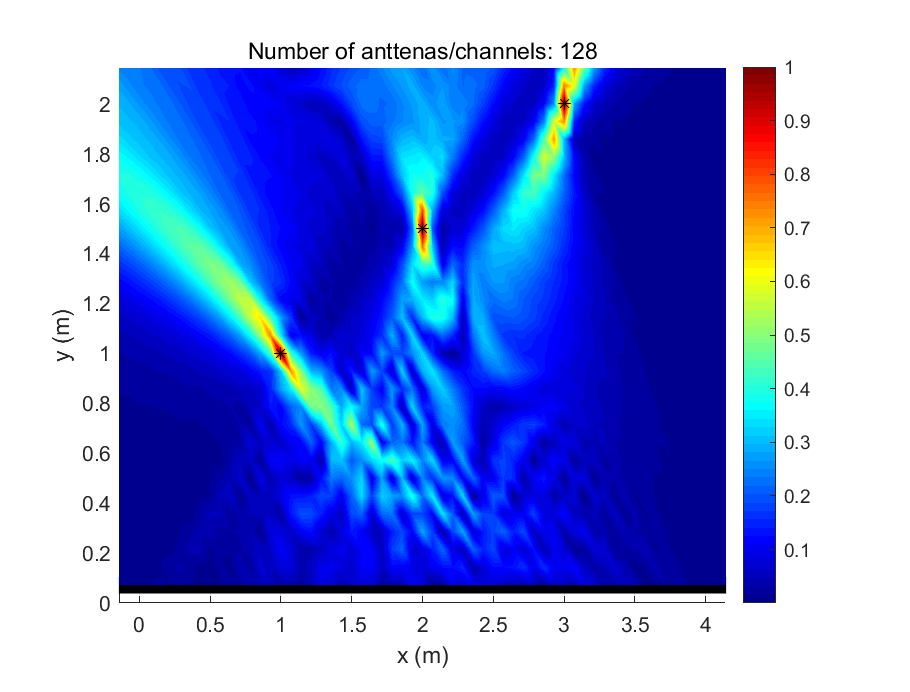
\includegraphics[width=1\textwidth]{figures/expected/128.eps}
      \caption{接收机天线阵元数$N=128$}
  \end{subfigure}
  \begin{subfigure}[t]{.45\linewidth}
      \centering
      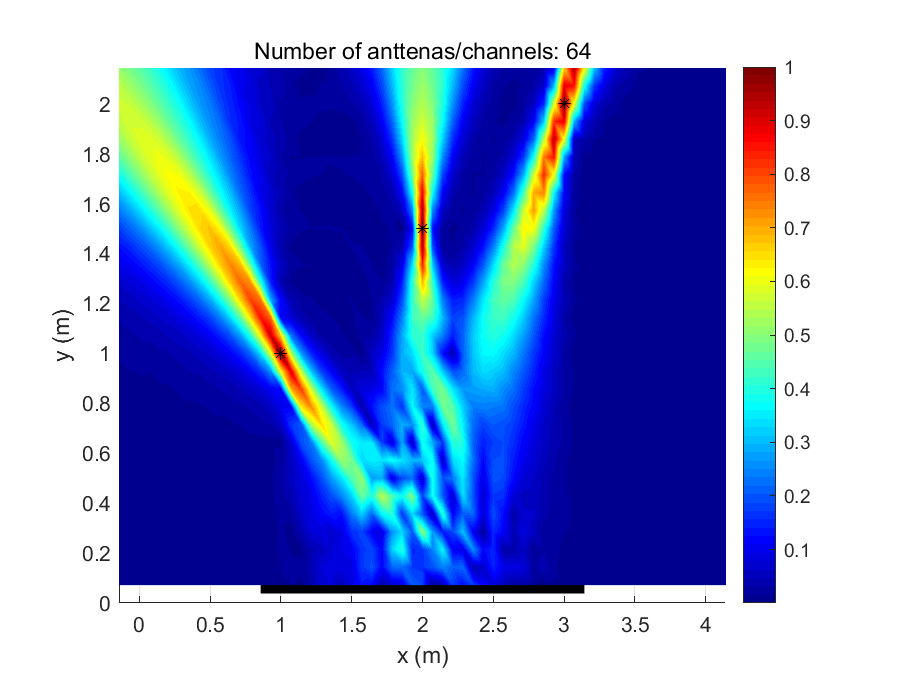
\includegraphics[width=1\textwidth]{figures/expected/64.eps}
      \caption{接收机天线阵元数$N=64$}
  \end{subfigure}
  \\
  \begin{subfigure}[t]{.45\linewidth}
    \centering
    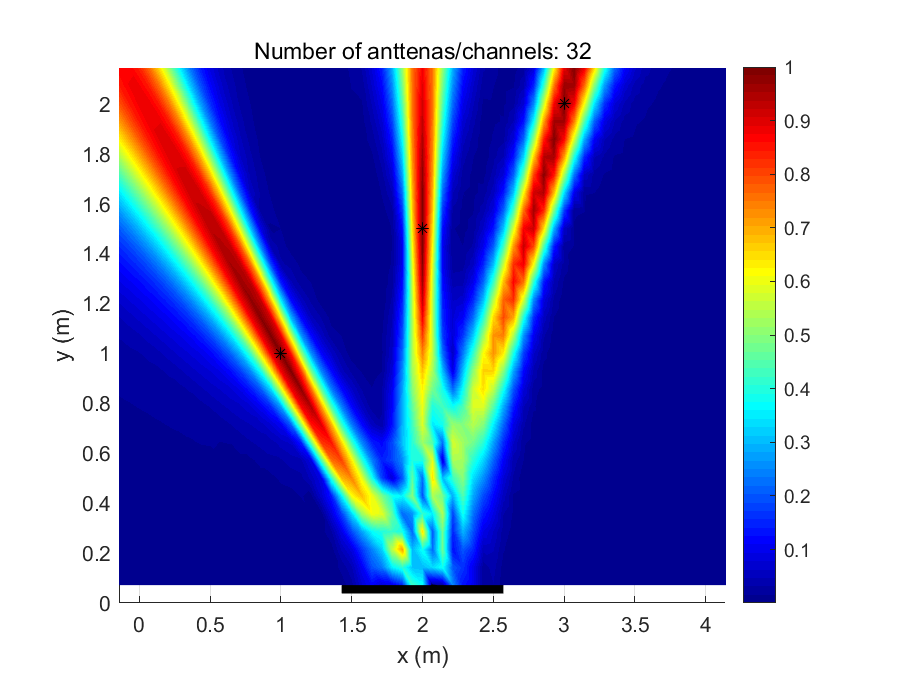
\includegraphics[width=1\textwidth]{figures/expected/32.eps}
    \caption{接收机天线阵元数$N=32$}
\end{subfigure}
  \caption{理想成像仿真结果}\label{理想成像仿真结果}
\end{figure}
仿真结果表明,理想的仿真成像可以良好的对目标进行检测,定位,和成像。